%!TEX root = ../dokumentation.tex

\chapter{Implementierung}

Dieses Kapitel beinhaltet sämtliche Implementierungen und Features in der App.
Dabei werden benutzte Libraries und Code aus der App gezeigt.

\section{App Tour}

Im Folgenden wird der Ablauf eines Bezahlvorgangs vom Start der App bis zu ihrer Beendigung dargestellt.\\
Beim Start der App wird man mit einem SplashScreen begrüßt.

\begin{figure}[H]
  \centering
  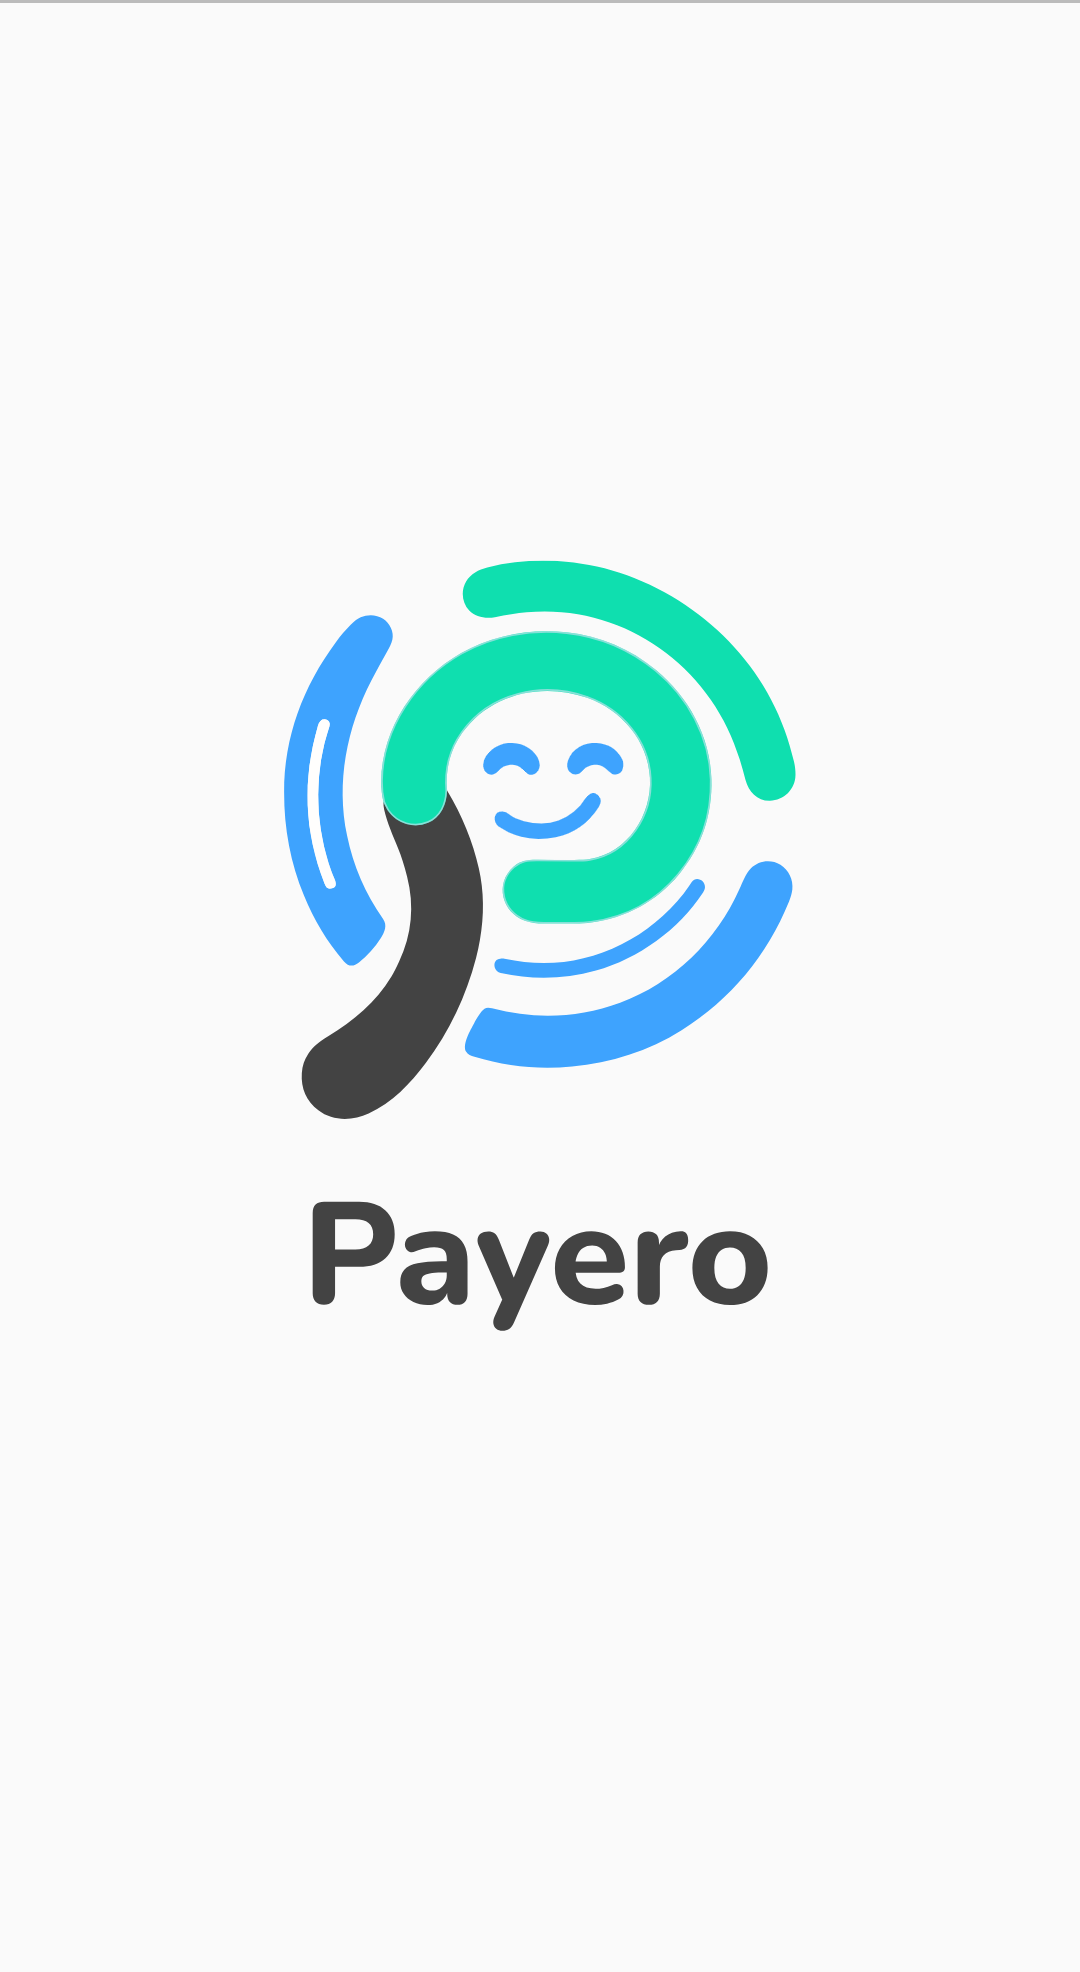
\includegraphics[width=.45\textwidth, height=.8\textwidth]{splashscreen.png}
  \caption{SplashScreen}
\end{figure}

Danach erfolgt beim ersten Start der Anwendung die Registrierung eines Benutzerkontos.
Dabei wird geprüft, ob die Felder ausgefüllt sind und ob eine E-Mail-Adresse im richtigen Format angegeben ist.
Dieser Schritt wird übersprungen, wenn bereits bei einer früheren Nutzung ein Benutzerkonto angelegt wurde.

\begin{figure}[H]
  \centering
  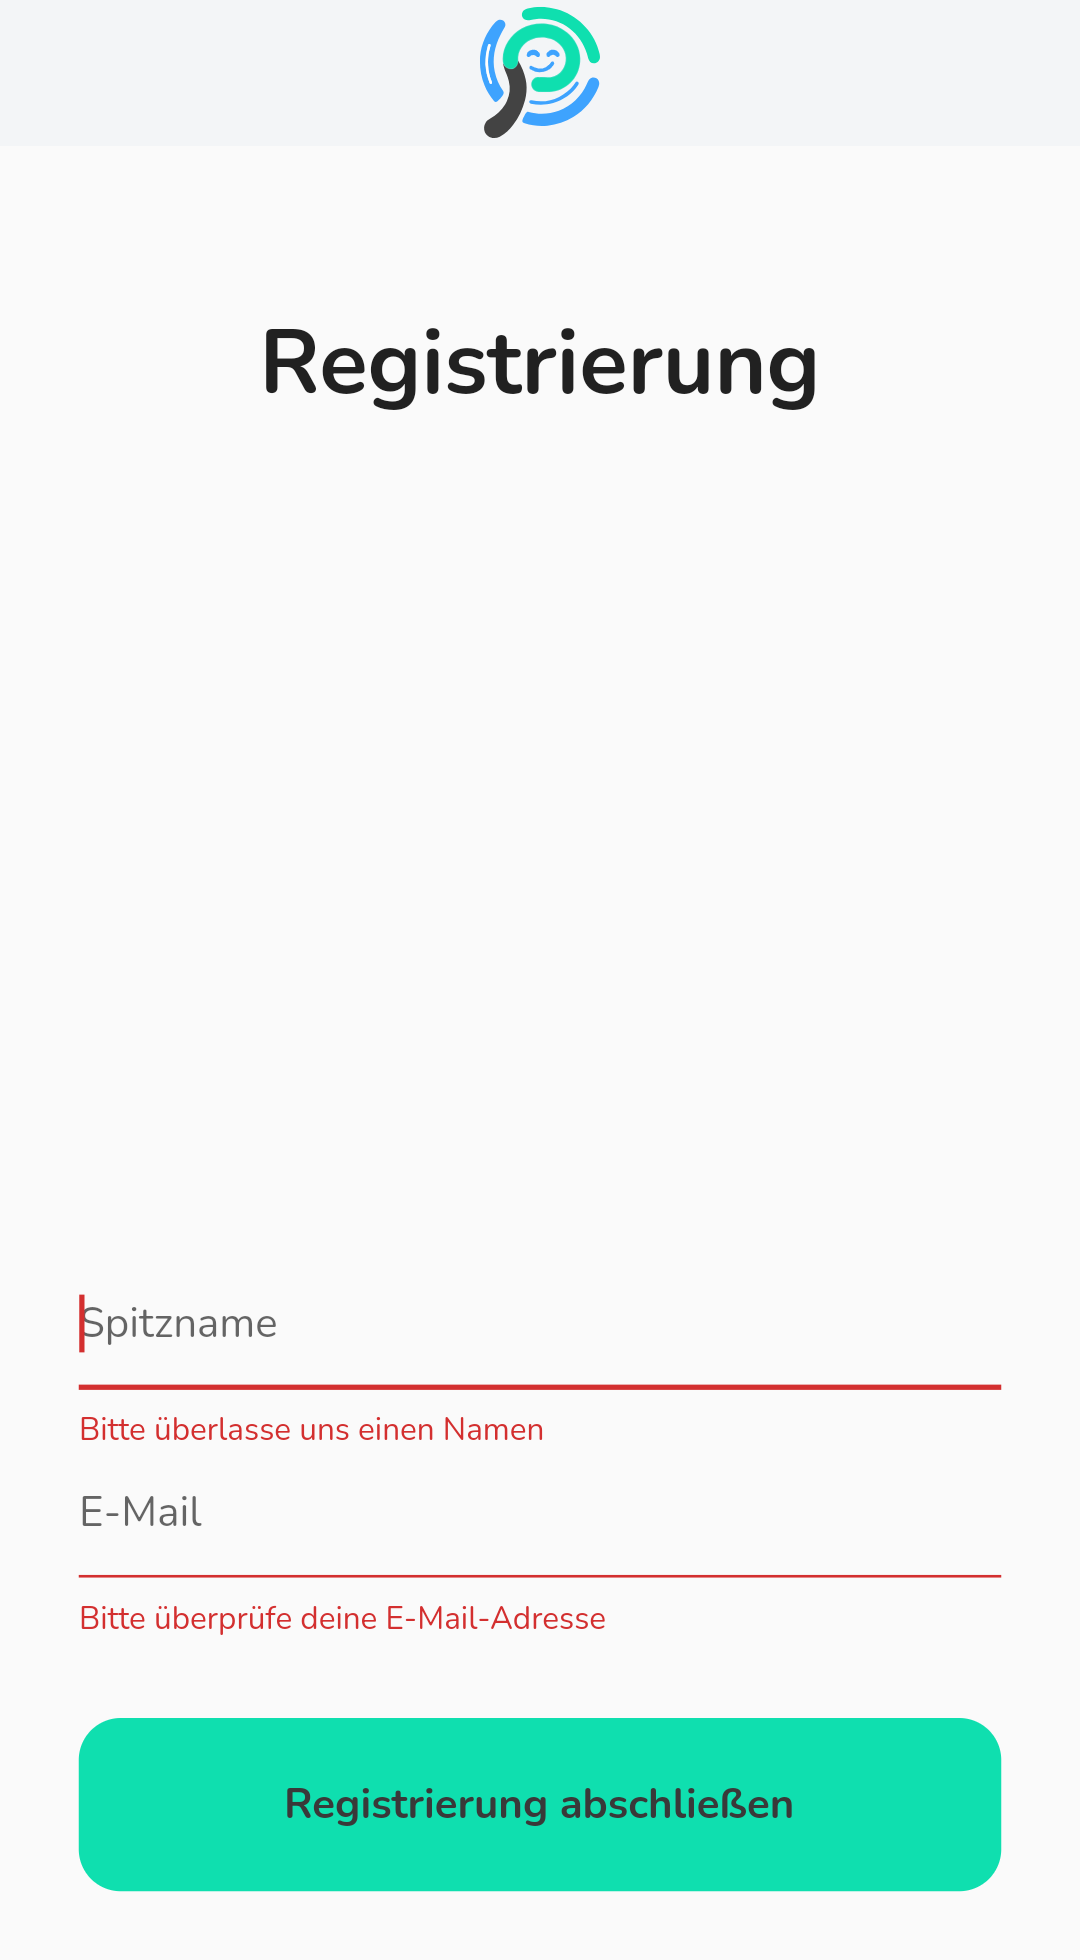
\includegraphics[width=.45\textwidth, height=.8\textwidth]{registration.png}
  \caption{Registrierungsvorgang}
\end{figure}

Danach gelangt man ins Hauptmenü.
Falls bereits ein Benutzerkonto besteht, gelangt man direkt nach dem SplashScreen ins Hauptmenü.

\begin{figure}[H]
  \centering
  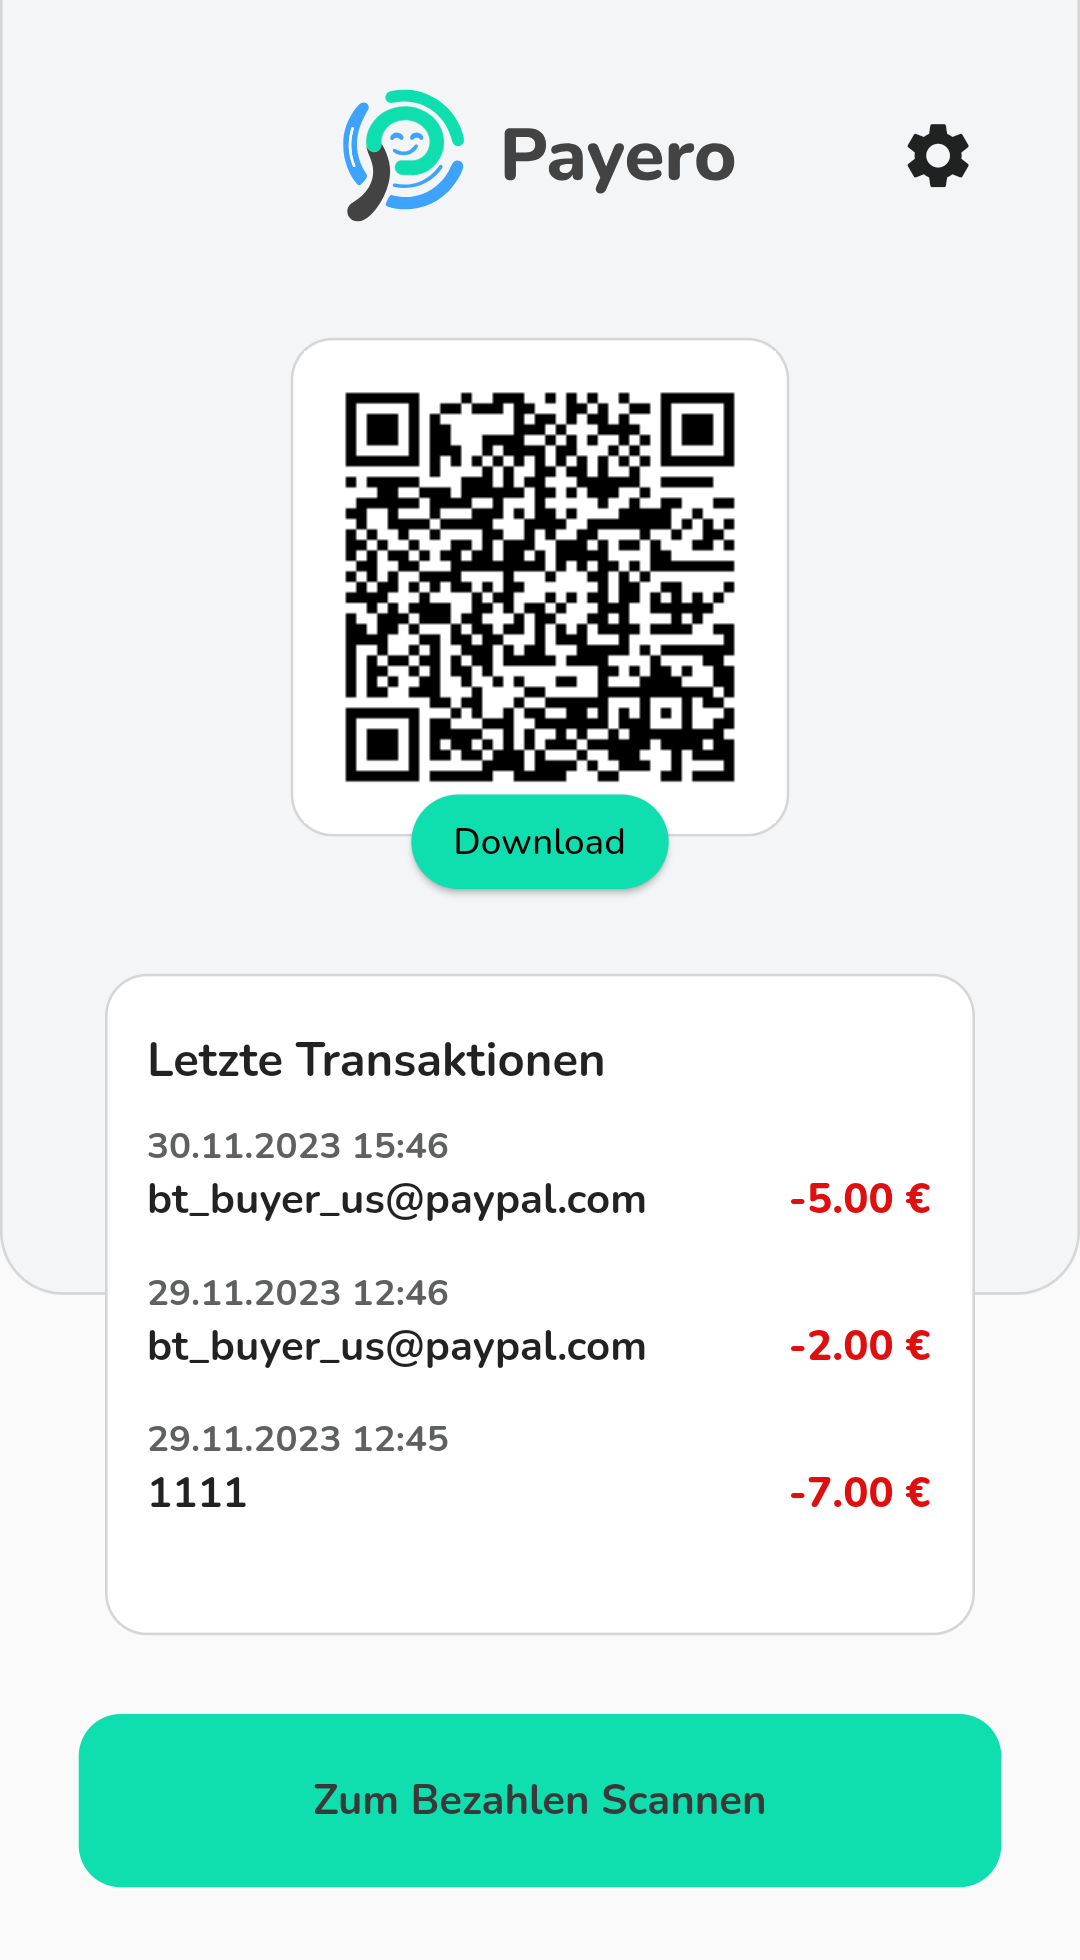
\includegraphics[width=.45\textwidth, height=.8\textwidth]{mainscreen_start.png}
  \caption{Hauptmenü}
\end{figure}

Im Hauptmenü finden Sie einen mit Ihrem Benutzerkonto verknüpften QR-Code, den Sie einscannen und herunterladen können.
Außerdem kann eine Transaktionshistorie mit den letzten drei Zahlungen eingesehen werden.
Ganz unten befindet sich ein Button.
Mit diesem wird der Bezahlvorgang gestartet.
In der rechten oberen Ecke befindet sich ein Icon für die Einstellungen.
Ein Klick darauf öffnet die Einstellungsseite.

\begin{figure}[H]
  \centering
  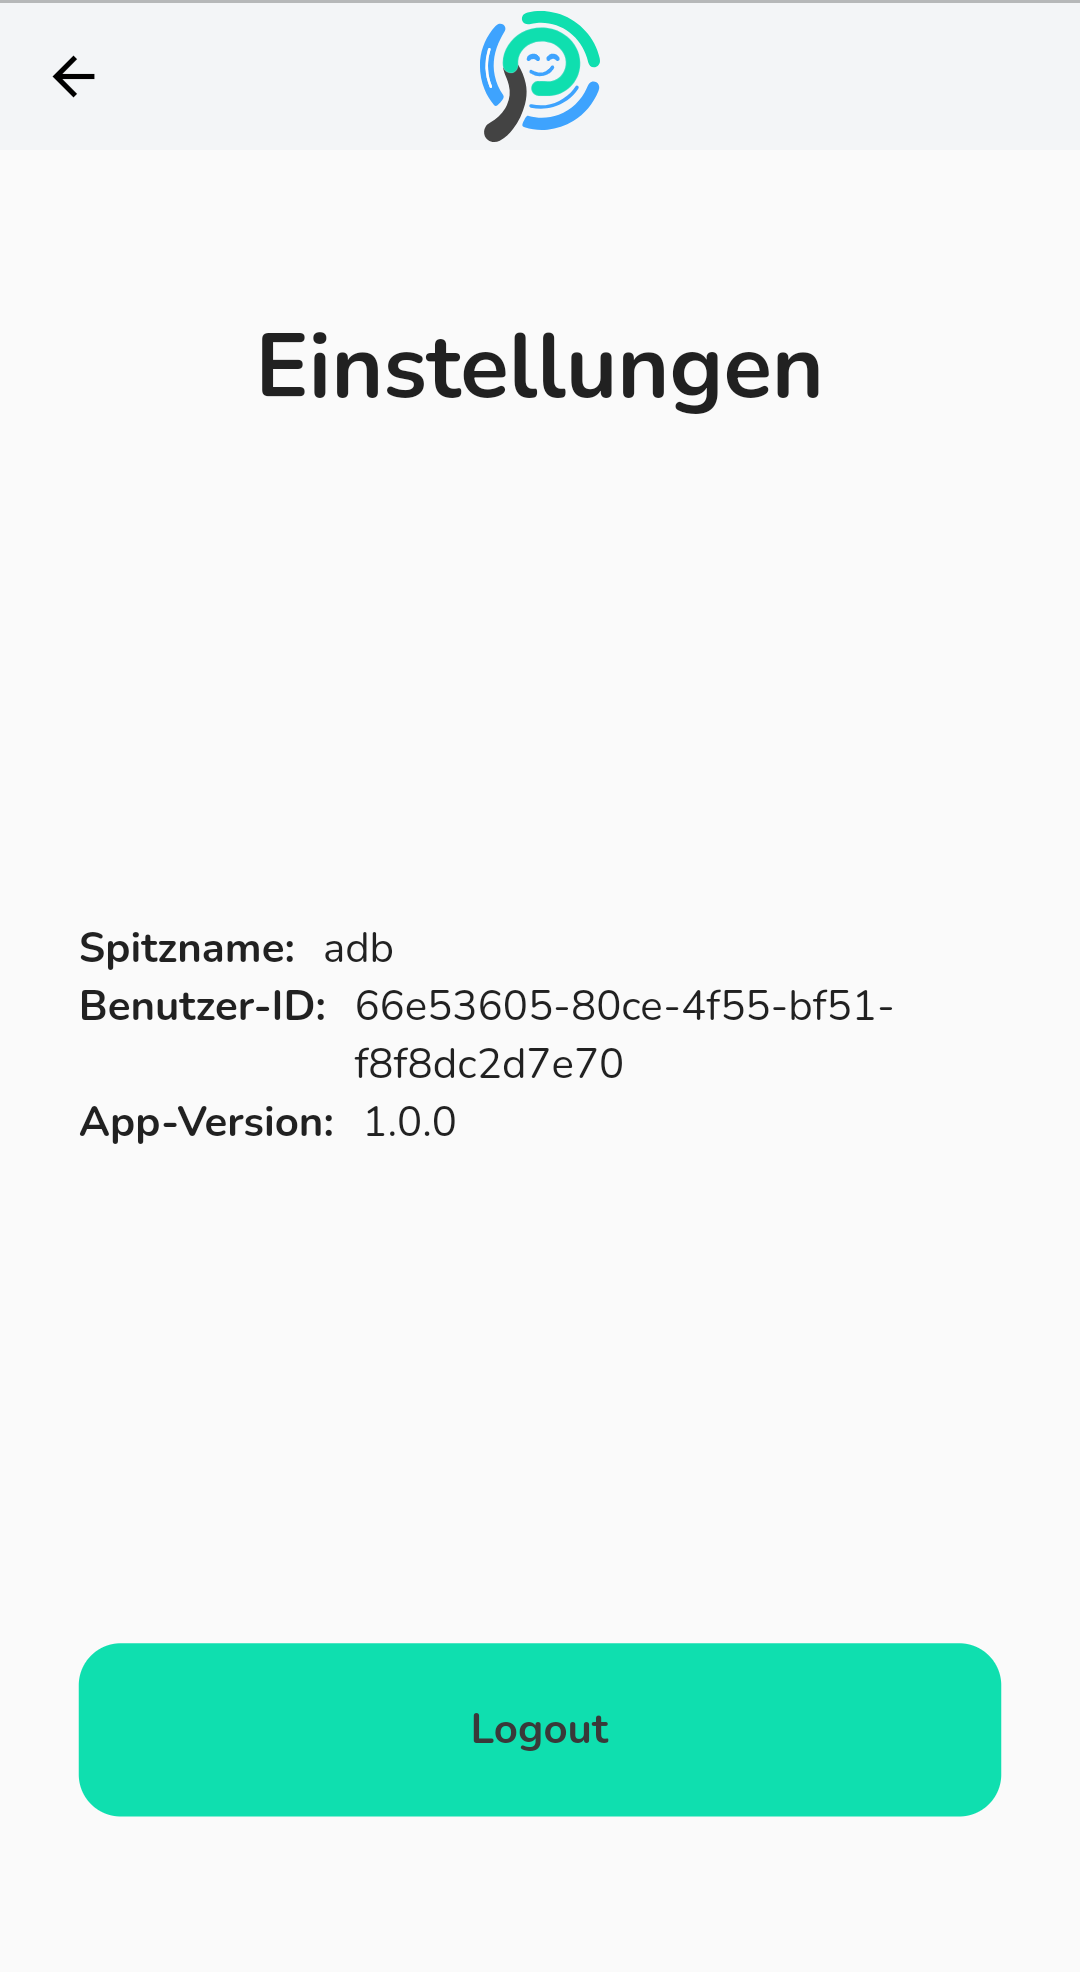
\includegraphics[width=.45\textwidth, height=.8\textwidth]{settings.png}
  \caption{Einstellungen}
\end{figure}

Auf der Einstellungsseite sieht man seinen Benutzernamen und die dazugehörige ID.
Auch die Version der Anwendung ist hier aufgelistet.
Man kann sich auch von seinem Benutzerkonto abmelden.
Geht man nun zurück ins Hauptmenü und startet den Bezahlvorgang mit einem Klick auf den Button, öffnet sich eine neue Seite.
Hier wird die Kameraberechtigung zum Einscannen eines QR-Codes abgefragt.
Dabei wird geprüft, ob es sich bei diesem QR-Code auch um einen Payero-QR-Code handelt.
Ist dies nicht der Fall, wird dies so angezeigt:

\begin{figure}[H]
  \centering
  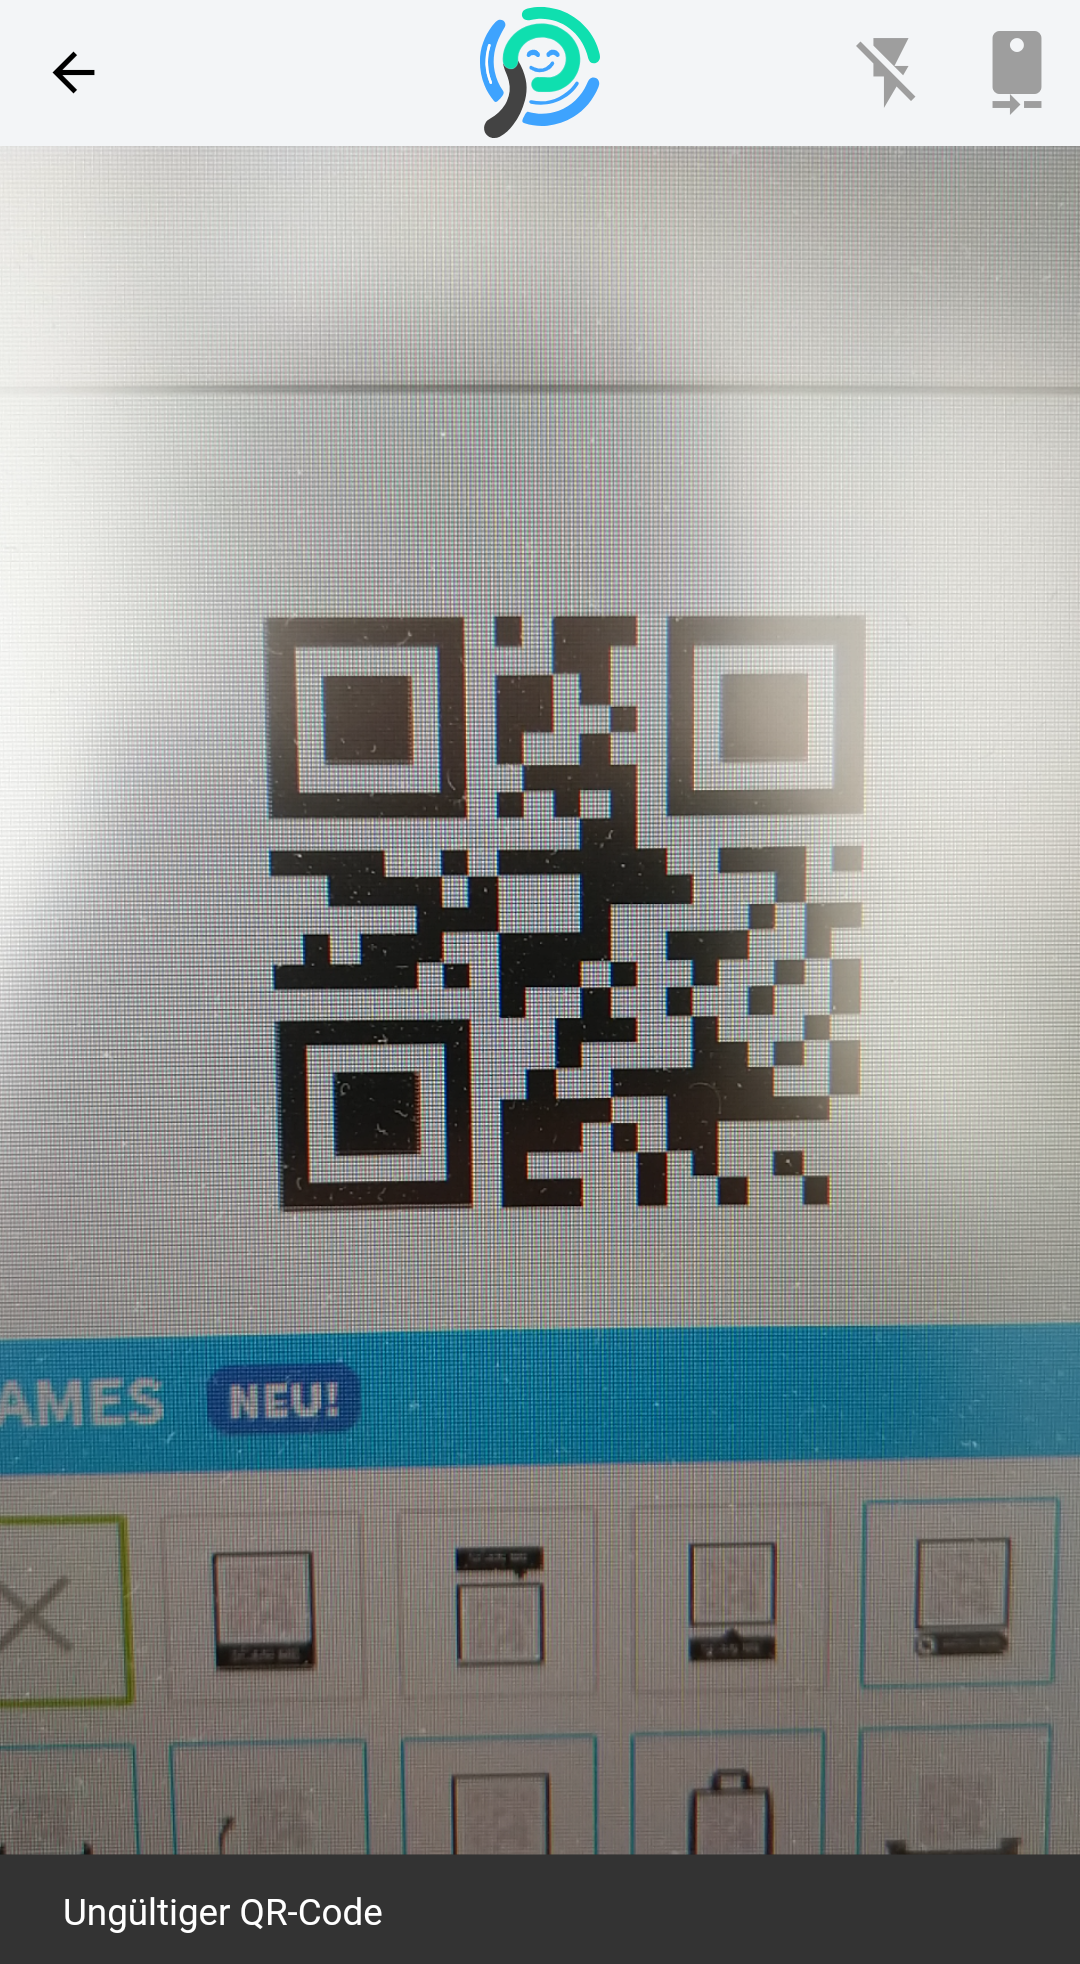
\includegraphics[width=.45\textwidth, height=.8\textwidth]{scan_wrong_qr.png}
  \caption{Ungültiger QR-Code}
\end{figure}

Eine SnackBar weist den Benutzer darauf hin, dass es sich nicht um einen gültigen QR-Code handelt.
Zusätzlich kann der Benutzer oben rechts durch Klick auf das entsprechende Icon den Kamerablitz aktivieren, falls es zu dunkel zum Scannen ist.
Es ist auch möglich, die Frontkamera zu aktivieren und zwischen dieser und der Rückkamera zu wechseln, indem man auf das entsprechende Symbol klickt.
Das Scannen eines QR-Codes erfolgt automatisch.
Der Benutzer muss dazu keine Schaltflächen anklicken.
Wird ein gültiger QR-Code erkannt, wird der Benutzer automatisch auf eine Bestätigungsseite weitergeleitet.

\begin{figure}[H]
  \centering
  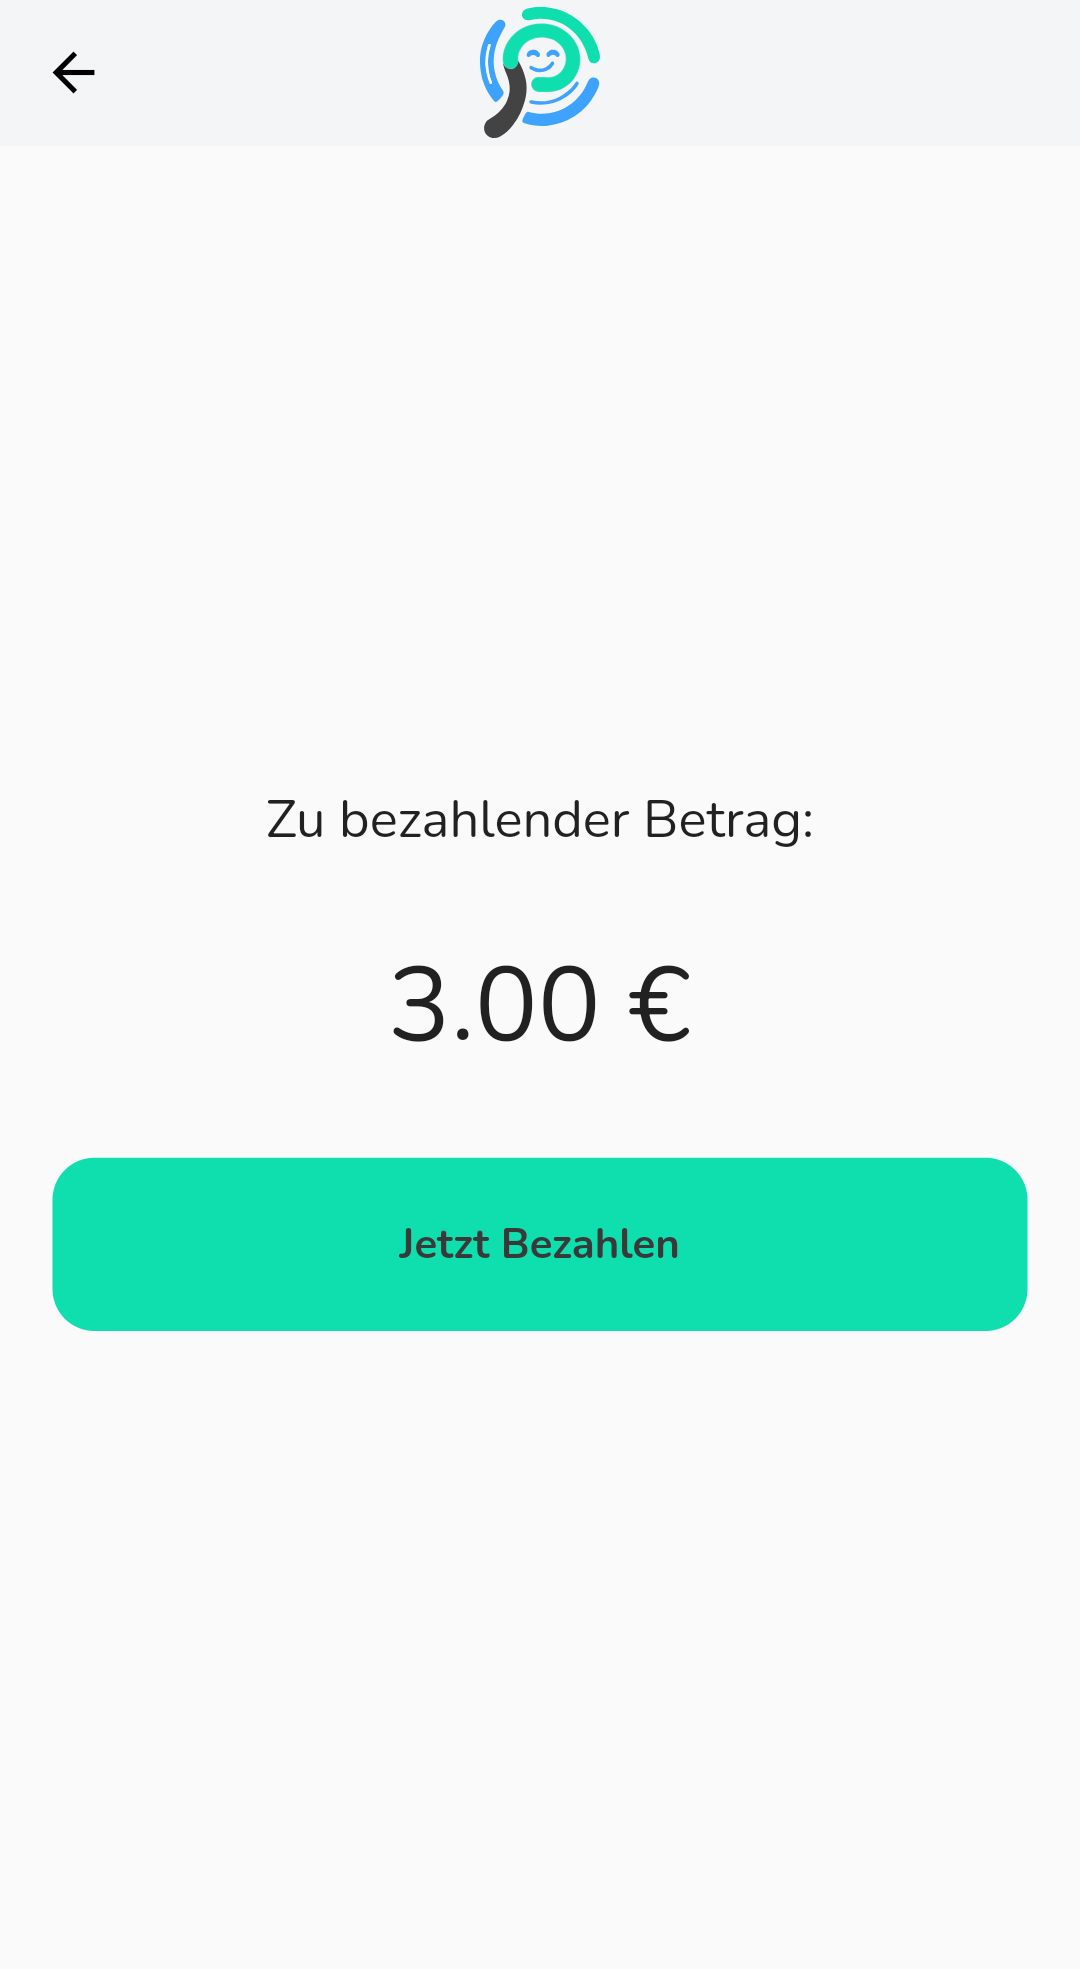
\includegraphics[width=.45\textwidth, height=.8\textwidth]{scan_good_qr.png}
  \caption{Bestätigungsseite}
\end{figure}

Auf dieser Seite wird der Benutzer über den zu zahlenden Betrag informiert.
Durch Anklicken des Buttons kann der Benutzer den Bezahlvorgang starten oder über den Zurück-Button abbrechen.
Beim Start des Bezahlvorgangs öffnet sich ein Dropin-Fenster.

\begin{figure}[H]
  \centering
  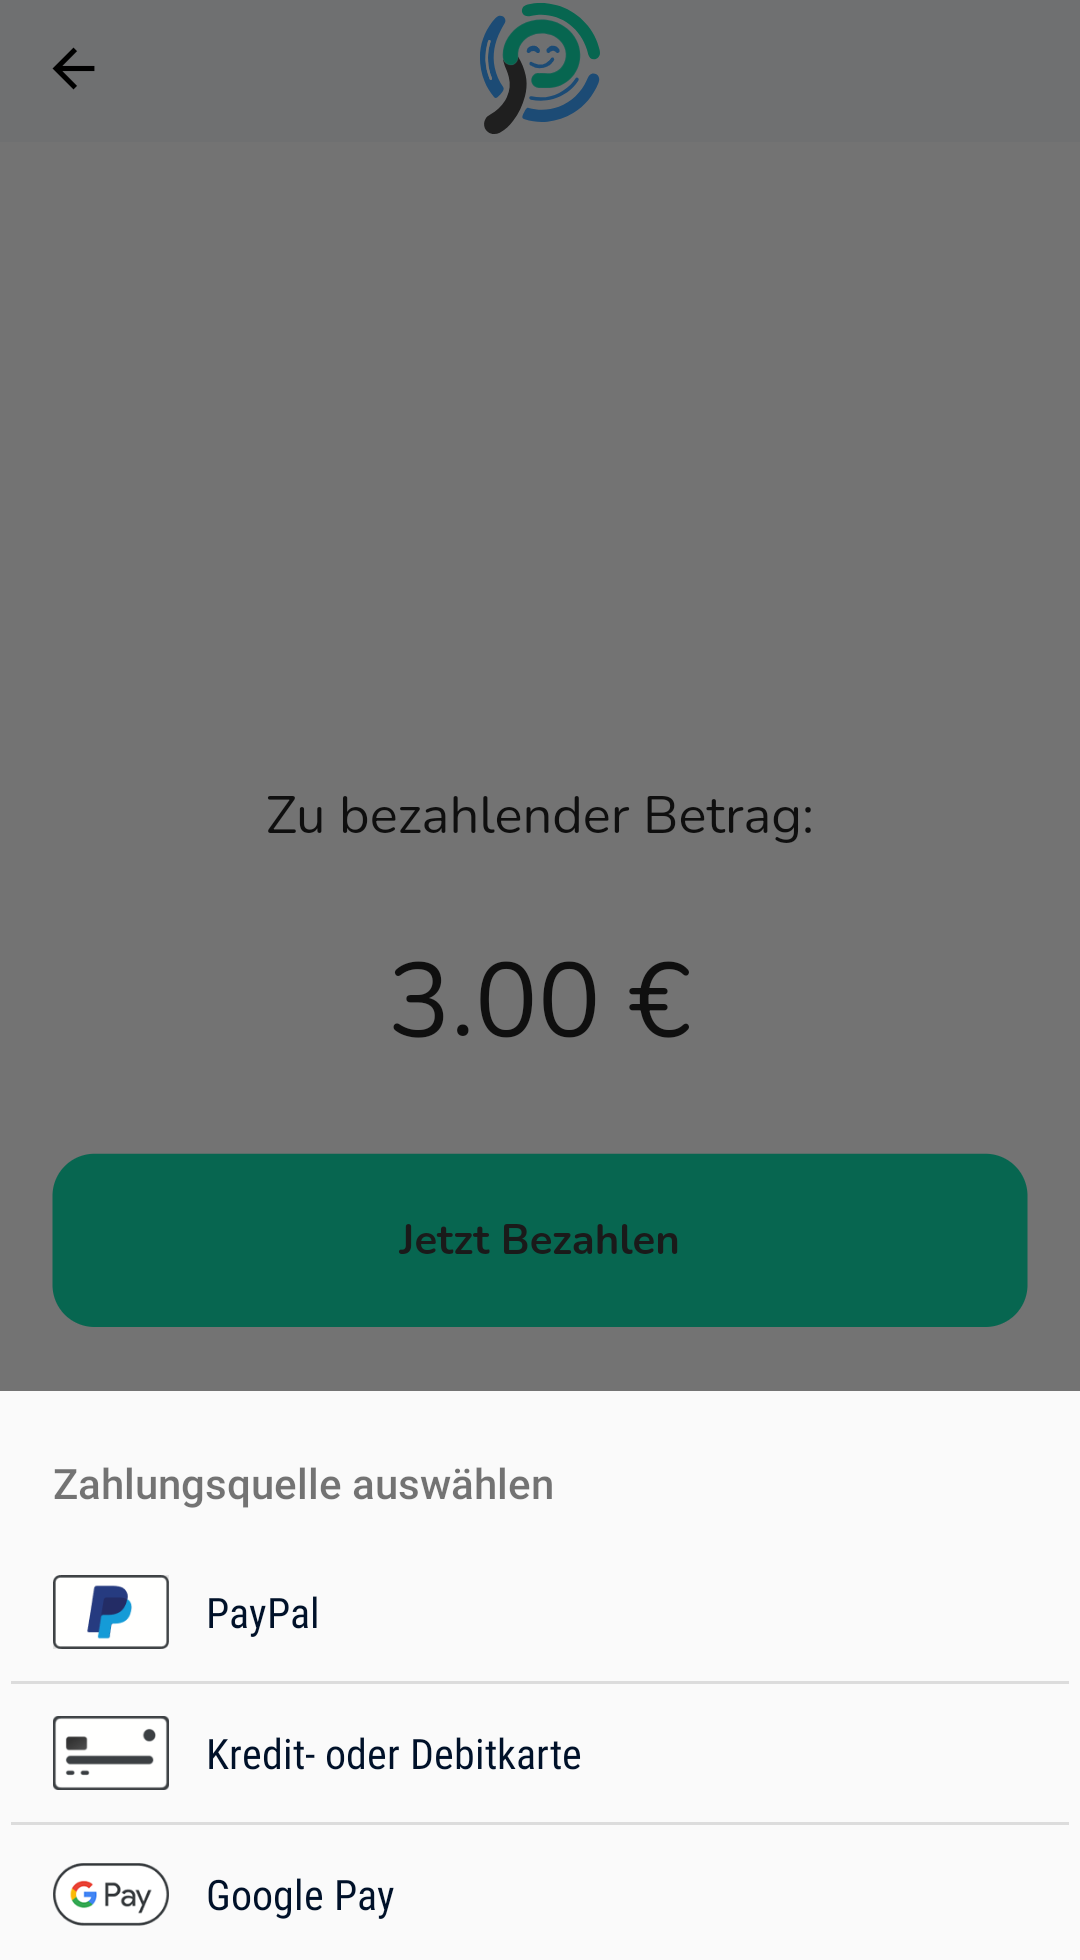
\includegraphics[width=.45\textwidth, height=.8\textwidth]{payment_option.png}
  \caption{Bezahlmethoden}
\end{figure}

Hier sieht der Benutzer alle verfügbaren Zahlungsmethoden.
Dazu gehören immer PayPal und Kreditkarte.
Unter Android gehört auch GooglePay dazu, während unter iOS ApplePay zwar möglich wäre, aber aufgrund des fehlenden Entwicklerkontos nicht zur Verfügung steht.
Je nach Bezahlmethode muss der Nutzer seine Kreditkartendaten oder andere Daten wie das PayPal-Konto eingeben.
Dabei wird auch geprüft, ob alles passt, z.B. das Ablaufdatum der Kreditkarte.
Im Fehlerfall wird der Benutzer darauf hingewiesen.
Auch jetzt ist es noch möglich, den Bezahlvorgang abzubrechen.
Der Benutzer wird darüber in einer SnackBar informiert.
Führt der Benutzer die Zahlung jedoch aus, wird er in einer SnackBar über die Verarbeitung der Zahlung informiert.
Diese SnackBar enthält immer die Zahlungsart und die Informationen dazu.
Bei PayPal wäre dies PayPal und die dazugehörige E-Mail.
Bei einer Kreditkarte ist es die Art der Kreditkarte und die Endziffern der Kreditkartennummer.
In diesem Beispiel ist es eine VISA Kreditkarte mit den Endziffern 1111.

\begin{figure}[H]
  \centering
  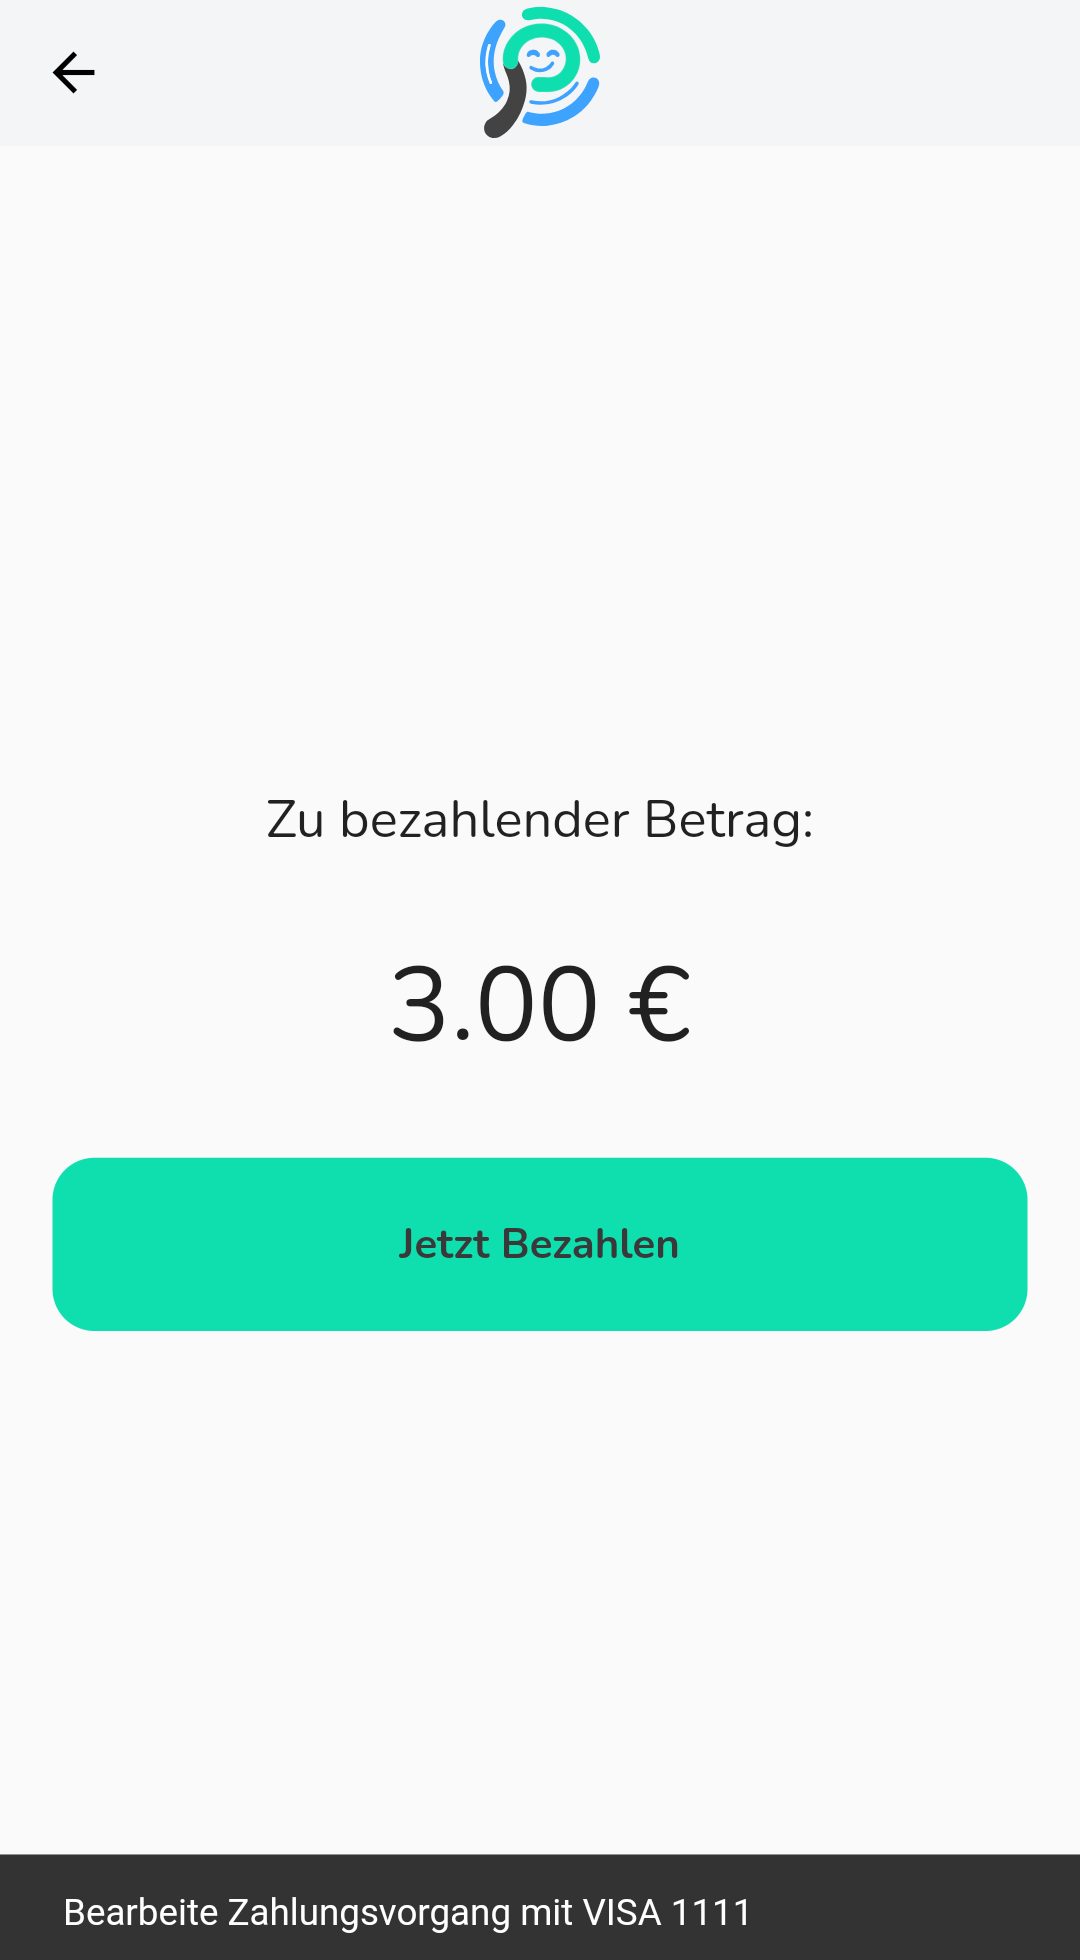
\includegraphics[width=.45\textwidth, height=.8\textwidth]{processing_payment.png}
  \caption{Verarbeitung des Bezahlvorganges}
\end{figure}

War der Vorgang erfolgreich, gelangt der Benutzer auf einen weiteren Bildschirm.
Dieser zeigt dem Benutzer an, dass die Zahlung erfolgreich durchgeführt wurde.
Außerdem wird der gezahlte Betrag angezeigt.

\begin{figure}[H]
  \centering
  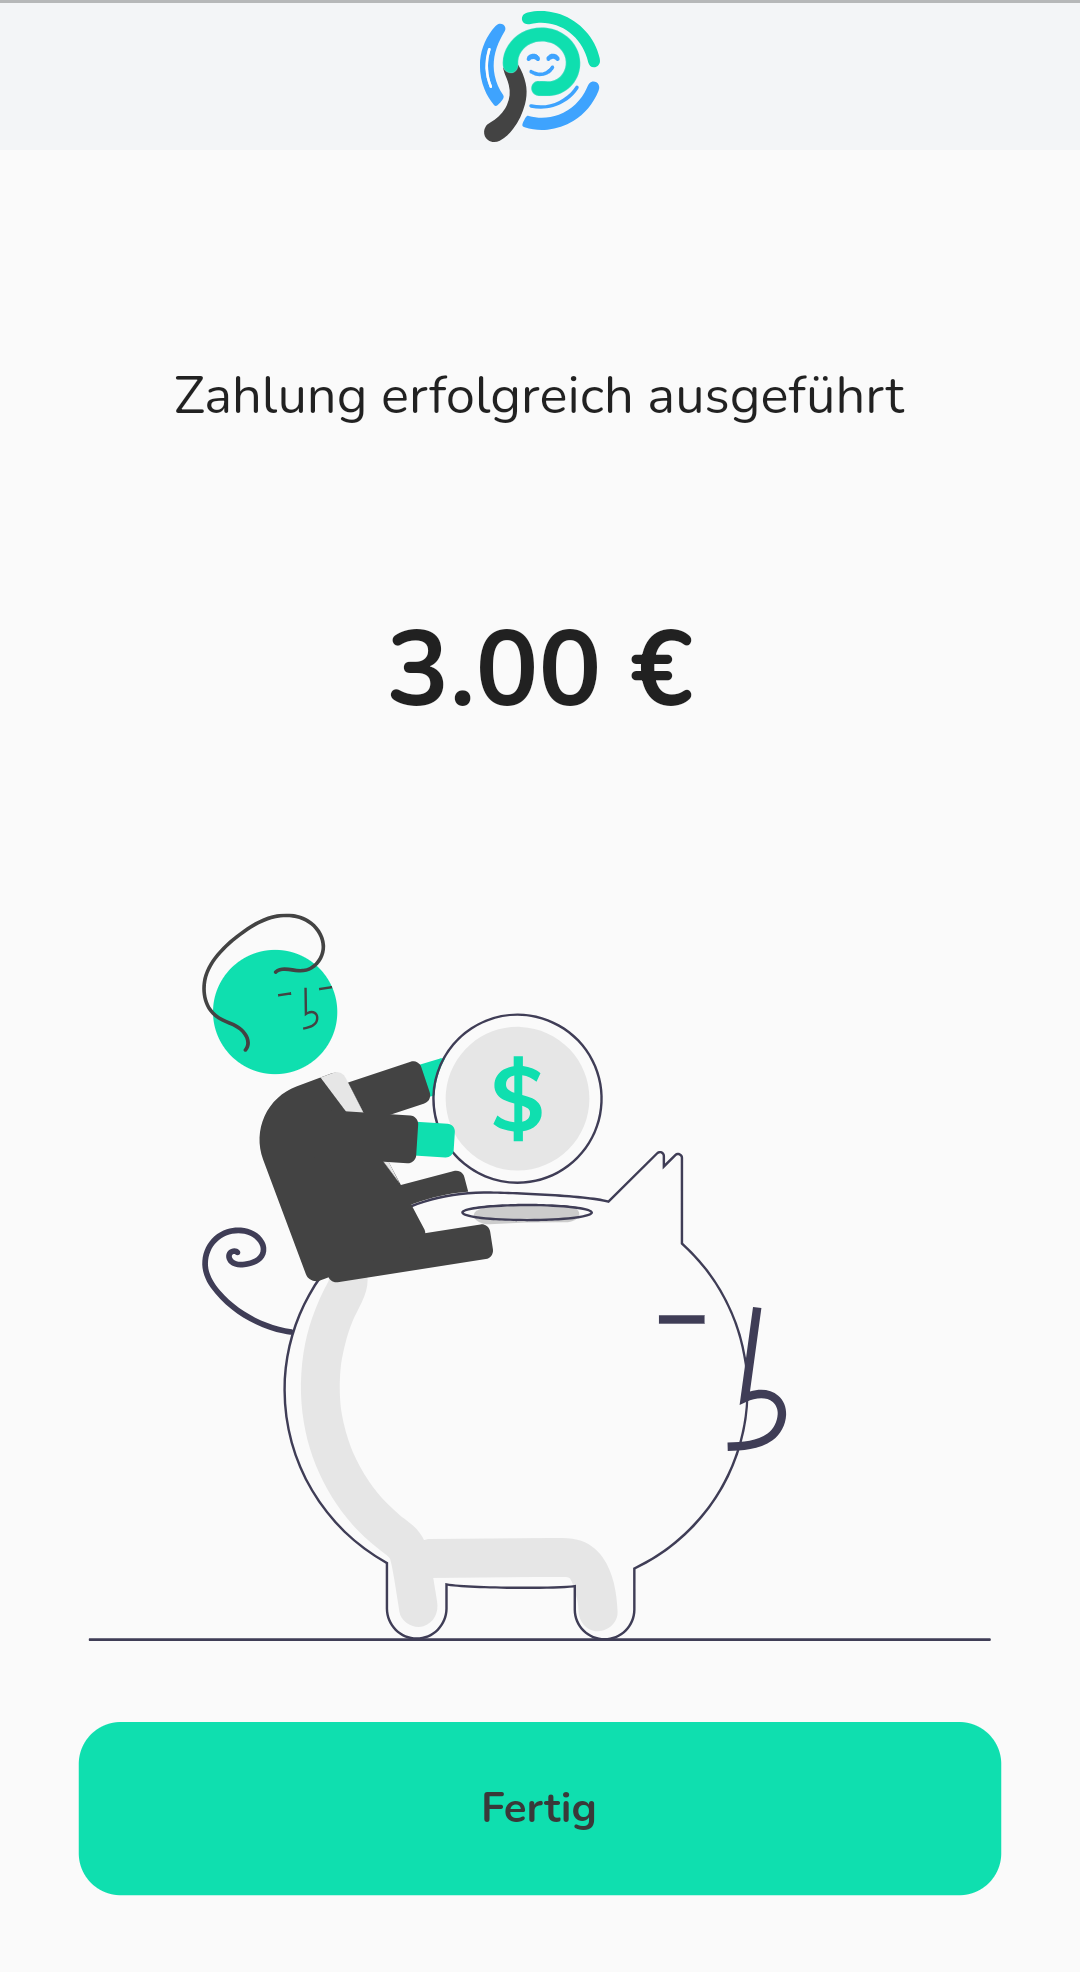
\includegraphics[width=.45\textwidth, height=.8\textwidth]{payment_success.png}
  \caption{Erfolgreicher Bezahlvorgang}
\end{figure}

Klickt der Benutzer auf den Button Fertig, gelangt er zurück zum Hauptmenü.
Dort ist in der Transaktionshistorie auch direkt ersichtlich, dass die Zahlung erfolgreich durchgeführt wurde.

\begin{figure}[H]
  \centering
  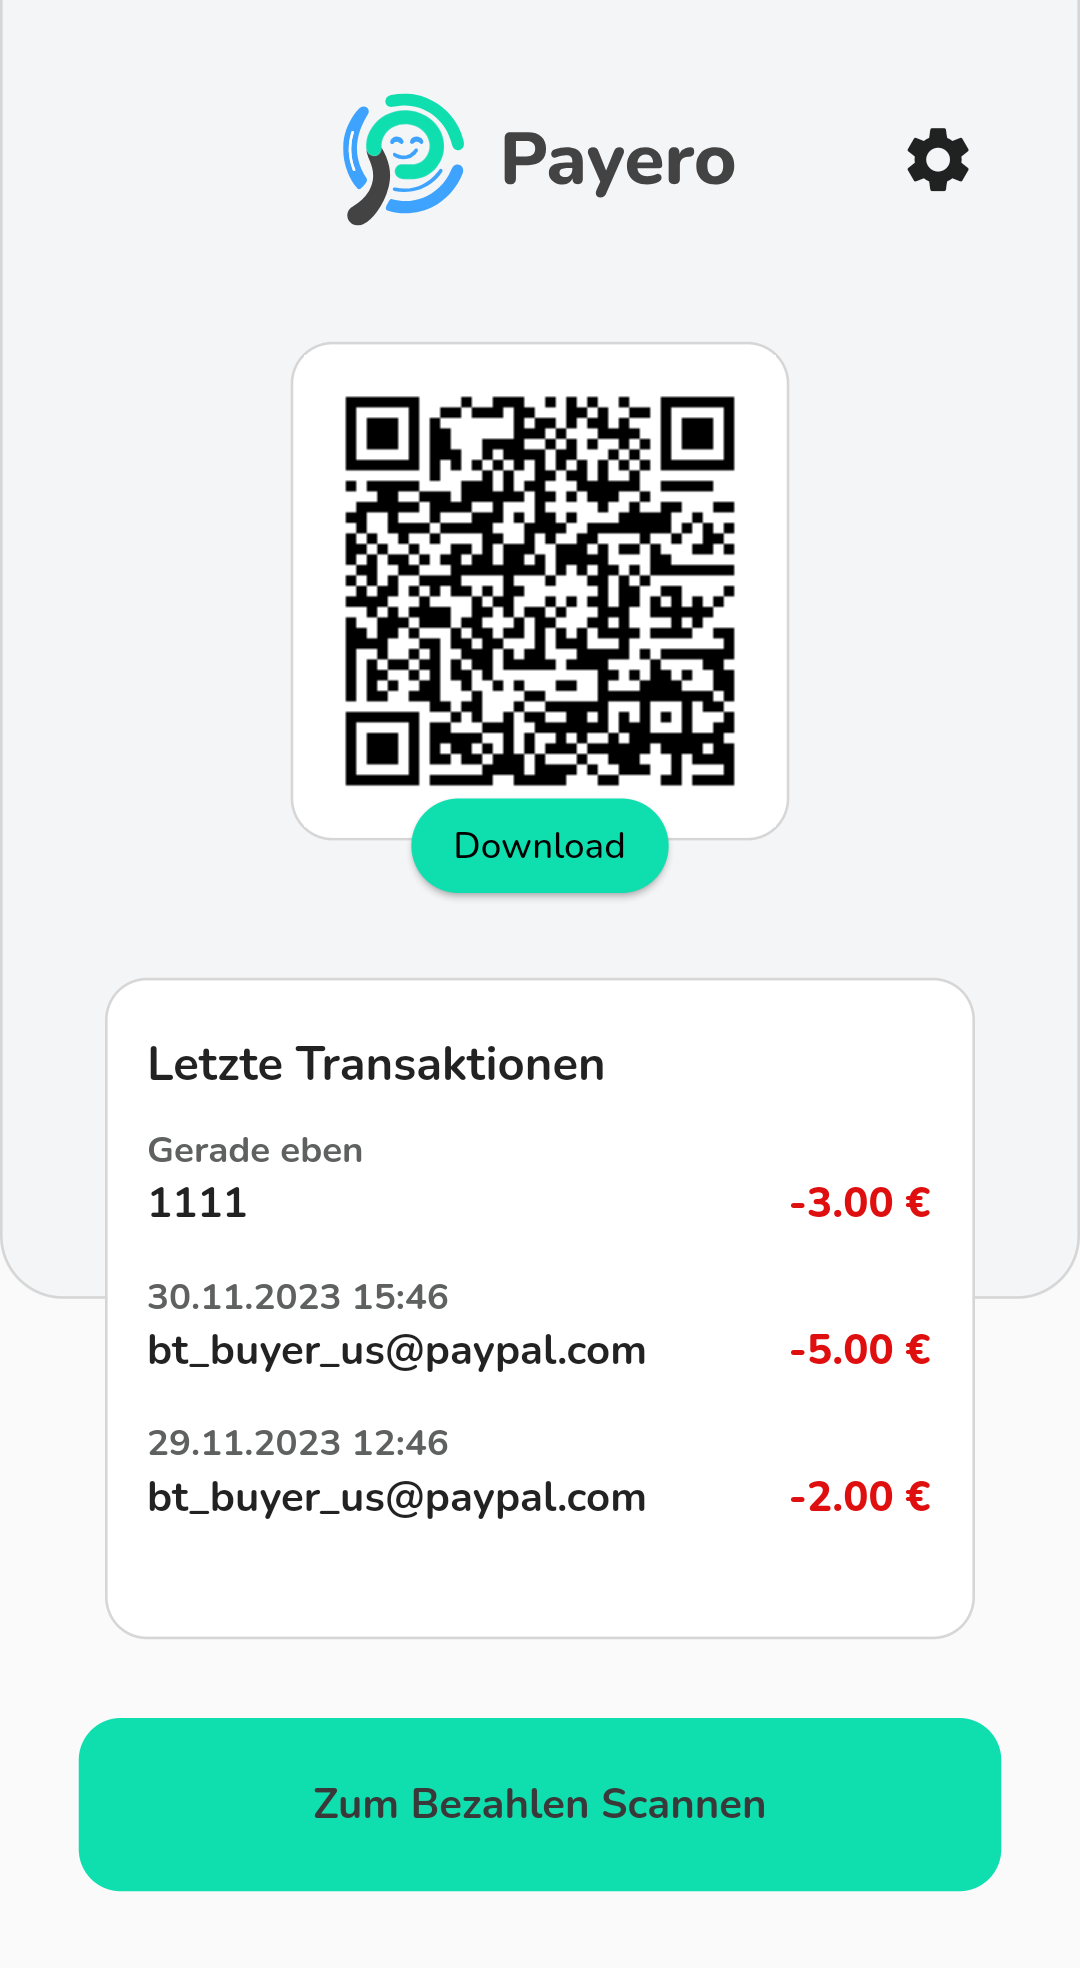
\includegraphics[width=.45\textwidth, height=.8\textwidth]{mainscreen_payment_success.png}
  \caption{Zahlung in der Transaktionshistorie sichtbar}
\end{figure}

Der Benutzer kann nun einen weiteren Bezahlvorgang starten.

\section{Transaktionshistorie}
Die Transaktionshistorie wurde komplett mithilfe von den zwei selbst entwickelten Widgets TransactionHistory und TransactionEntry implementiert.
Diese sind beide stateless, bekommen ihre Inhalte also vom MainScreen in Form eines Arrays übergeben.\\
Die TransactionHistory stellt mithilfe der take()-Funktion die ersten drei Einträge des übergebenen Arrays dar, wodurch nur die aktuellsten Transaktionen angezeigt werden.
Sofern keine Transaktionen vorhanden sind, wird ein Text dargestellt.\\
Im TransactionEntry wird ein Eintrag mit dem Zeitstempel der Transaktion, der Beschreibung und dem Betrag gerendert.
Ausgehende Transaktionen stellen negative Werte dar und werden in roter Farbe dargestellt.
Andernfalls werden die Beträge grün dargestellt.\\
Bei der Überweisung per Kreditkarte kam es zu dem Problem, dass sehr lange Beschreibungstexte abgespeichert wurden.
Um ein horizontales Überlaufen zu verhindern, wird der Text daher nach 20 Zeichen abgeschnitten.\\
Ebenfalls wurde eingebaut, dass die Zeitstempel formatiert je nach Alter als etwa „Gerade eben“, „Vor 24 Minuten“, „16:43 Uhr“ oder im Format „23.11.2023 16:00“ ausgegeben werden.
Das Verhalten wird in Abbildung \ref{fig:transactionhistory} dargestellt.

\begin{figure}[H]
  \centering
  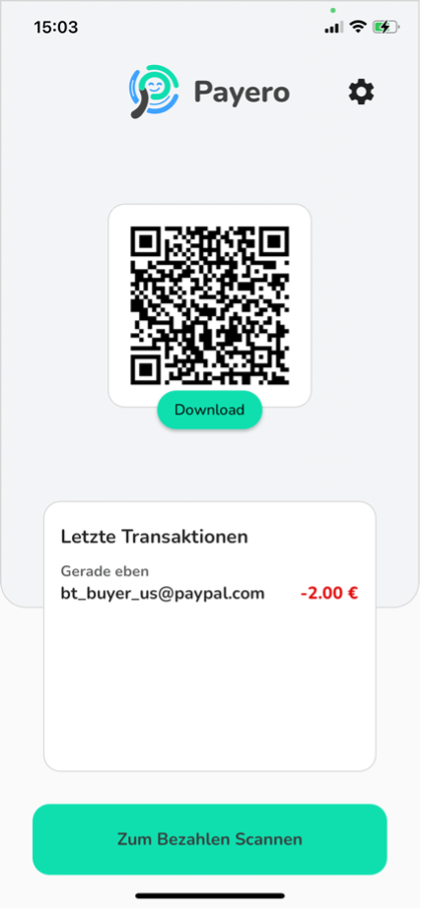
\includegraphics{onetransaction.png}
  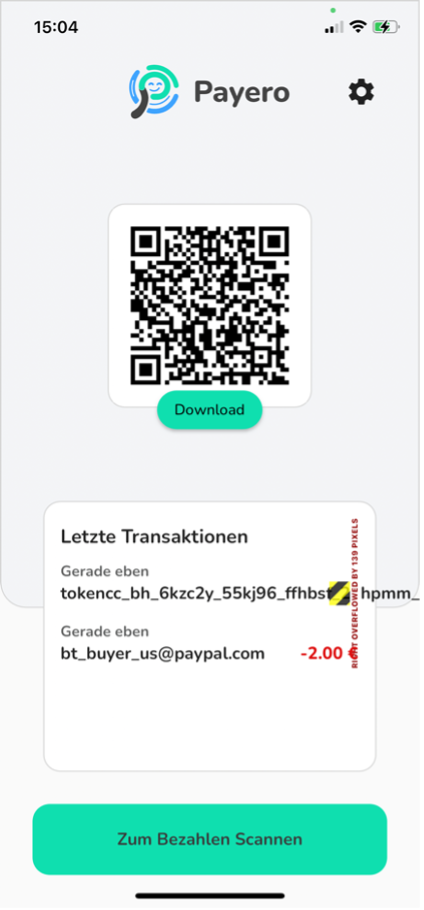
\includegraphics{overflowingtransaction.png}
  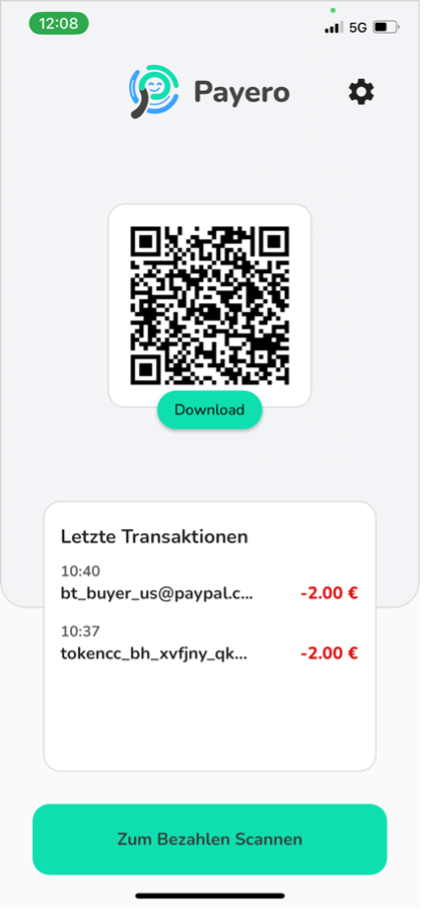
\includegraphics{multipletransactions.png}
  \caption{Darstellung der Transaktionshistorie in verschiedenen Fällen, mit einer Transaktion, ohne Textkürzung, und mit mehreren Transaktionen.}
  \label{fig:transactionhistory}
\end{figure}

\section{QR-Code Scanner}

Zum Erkennen und Scannen der QR-Codes wird die Library \glqq mobile\_scanner\grqq{} in der Version \glqq 3.5.2\grqq{} genutzt.
Diese arbeitet sowohl unter iOS als auch Android zuverlässig.
Die Integration findet in der \glqq qr\_code\_scan\_screen.dart\grqq{} Datei statt.
Es wird hierzu die Klasse \glqq \_QRScanScreenState\grqq{} erstellt in welcher die Funktionen der Library implementiert werden.
Unter anderem ist hier die Steuerung der Kamera, das Umschalten zwischen Front- und Rückkamera und die Steuerung des Kamerablitzes möglich.

\begin{lstlisting}[caption=Kamerasteuerung, label=cam_ctrl]
	appBar: PayeroHeader(showBackButton: true, actions: [
        IconButton(
          color: Colors.white,
          icon: ValueListenableBuilder(
            valueListenable: cameraController.torchState,
            builder: (context, state, child) {
              switch (state as TorchState) {
                case TorchState.off:
                  return const Icon(Icons.flash_off, color: Colors.grey);
                case TorchState.on:
                  return const Icon(Icons.flash_on, color: Colors.yellow);
              }
            },
          ),
          iconSize: 32.0,
          onPressed: () => cameraController.toggleTorch(),
        ),
        IconButton(
          color: Colors.white,
          icon: ValueListenableBuilder(
            valueListenable: cameraController.cameraFacingState,
            builder: (context, state, child) {
              switch (state as CameraFacing) {
                case CameraFacing.front:
                  return const Icon(Icons.camera_front, color: Colors.grey);
                case CameraFacing.back:
                  return const Icon(Icons.camera_rear, color: Colors.grey);
              }
            },
          ),
          iconSize: 32.0,
          onPressed: () => cameraController.switchCamera(),
        )
      ])
\end{lstlisting}

Der Scan wird mit einer kurzen Verzögerung gestartet, um sicherzustellen, dass alles vollständig geladen ist.
Die erfolgreich gescannten Barcodes und QR-Codes werden als Liste gespeichert.
Wir verwenden hier aber immer nur den ersten erfolgreichen Code in der Liste.

\begin{lstlisting}[caption=QR-Code gefunden, label=qr_found]
  body: MobileScanner(
        startDelay: true,
        controller: cameraController,
        onDetect: (capture) {
          final List<Barcode> barcodes = capture.barcodes;
          if (barcodes.isNotEmpty && !_screenOpened) {
            final String code = barcodes.first.rawValue ?? "---";
            debugPrint('QRCode found! $code');
\end{lstlisting}

Nun wird geprüft, ob der gescannte QR-Code ein gültiges Format hat, andernfalls wird er abgelehnt.
Der Benutzer wird darüber in einer SnackBar informiert.

\begin{lstlisting}[caption={QR-Code Check}]
  try {
    final Map<String, dynamic> data = jsonDecode(code);

    // Ueberpruefen, ob der Namespace 'payero' ist
    if (data['namespace'] != 'payero') {
      ScaffoldMessenger.of(context).showSnackBar(
        const SnackBar(content: Text('Ungueltiger QR-Code')),
      );
      return; // Beenden der Funktion, wenn der Namespace nicht stimmt
    }

    // Ueberpruefen, ob der 'amount' zu einem double konvertiert werden kann
    final double? amount = double.tryParse(data['amount'].toString());
    if (amount == null) {
      ScaffoldMessenger.of(context).showSnackBar(
        const SnackBar(content: Text('Ungueltiger QR-Code')),
      );
      return; // Beenden der Funktion, wenn der amount ungueltig ist
    }

    final String formattedAmount = amount.toStringAsFixed(2);

    ScaffoldMessenger.of(context).removeCurrentSnackBar();

    // Weitermachen mit gueltigen Daten
    _screenOpened = true;
    Navigator.push(
      context,
      MaterialPageRoute(
        builder: (context) => FoundCodeScreen(
          screenClosed: _screenWasClosed,
          userId: userId,
          value: formattedAmount,
        ),
      ),
    ).then((_) => _screenWasClosed());
  } catch (e) {
    debugPrint("Error while scanning: ${e.toString()}");
    // Generische Fehlermeldung anzeigen
    ScaffoldMessenger.of(context).showSnackBar(
      const SnackBar(content: Text('Ungueltiger QR-Code')),
    );
  }
\end{lstlisting}

Das gültige Format eines QR-Codes ist JSON und sieht wie folgt aus:

\begin{lstlisting}[caption={Gültiger QR-Code}]
  {
   "namespace":"payero",
   "userID":"user1",
   "amount":"3.00"
  }
\end{lstlisting}

Der entsprechende QR-Code sieht dann so aus:

\begin{figure}[H]
  \centering
  
\includegraphics[width=.3\textwidth, height=.3\textwidth]{qr-code.png}
  \caption{Gültiger QR-Code}
\end{figure}

Bei der Anzeige des Betrags innerhalb der App wird der Betrag auf jeder Seite nur mit zwei Nachkommastellen angezeigt.
Dies ist unabhängig davon, ob der \glqq amount\grqq{} im QR-Code Nachkommastellen enthält oder nicht, und dient ausschließlich kosmetischen Zwecken, verbessert aber aufgrund der immer gleichen Formatierung das Nutzererlebnis.
Dies gilt auch für die QR-Codes, die im Hauptmenü gescannt werden können.
Um zu verhindern, dass immer weiter gescannt wird, wenn ein QR-Code gefunden wurde, wird über den Parameter \glqq \_screenOpened\grqq{} ein Bool-Flag gesetzt.
Danach wird bei einem gültigen QR-Code auf eine neue Seite gewechselt.
Diese zeigt den zu zahlenden Betrag und einen Button, mit dem bezahlt werden kann.
Ein Klick auf den Button öffnet das BrainTree Dropin-UI.

\section{Bezahlintegration mit Braintree}

Die Zahlungsmethode kann im BrainTree Dropin-UI ausgewählt werden.
Derzeit werden PayPal, Kreditkarte (VISA, Mastercard) und GooglePay angeboten.
ApplePay ist ebenfalls implementiert, jedoch muss eine gültige Merchant-ID angegeben werden, um die Funktion zu aktivieren.
Diese Merchant-ID ist nur mit einer Mitgliedschaft im Apple Developer Program erhältlich.
Darüber hinaus wird ausschließlich der Sandbox-Account von Braintree genutzt, da es als Privatperson ohne gültige Umsatzsteuer-Identifikationsnummer und wahrheitsgemäße Angaben zu den Eigentumsverhältnissen oder der Stellung im Unternehmen gemäß \S\S 10 bis 17 Geldwäschegesetz nicht möglich ist, einen Produktiv-Account zu erhalten.
Ist man im Besitz eines gültigen Braintree-Produktivaccounts, muss lediglich der \glqq tokenizationKey\grqq{} ausgetauscht werden, um die Anwendung produktiv zu schalten.

\begin{lstlisting}[caption={BrainTree Bezahlmethoden}]
  class _FoundCodeScreenState extends State<FoundCodeScreen> {
  String currency = "EUR";

  void startBraintreeCheckout() async {
    var request = BraintreeDropInRequest(
      tokenizationKey:
          'sandbox_d53t3dpq_8fxhdjy2nrd33mtm', // Ersetzen mit echtem tokenizationKey aus BrainTree Account
      collectDeviceData: true,
      paypalRequest: BraintreePayPalRequest(
        amount: widget.value,
        displayName: 'Payero',
        currencyCode: currency,
      ),
      googlePaymentRequest: BraintreeGooglePaymentRequest(
        totalPrice: widget.value,
        currencyCode: currency,
        billingAddressRequired: false,
      ),
      applePayRequest: BraintreeApplePayRequest(
        paymentSummaryItems: [
          ApplePaySummaryItem(
              label: 'Payero',
              amount: double.parse(widget.value),
              type: ApplePaySummaryItemType.final_)
        ],
        displayName: 'Payero',
        currencyCode: currency,
        countryCode: 'DE',
        merchantIdentifier:
            'merchant.com.example.mobile_computing_payment_app', // Ersetzen mit echtem Apple Pay Merchant Identifier
        supportedNetworks: [
          ApplePaySupportedNetworks.visa,
          ApplePaySupportedNetworks.masterCard,
          ApplePaySupportedNetworks.amex
        ],
      ),
      // Weitere Optionen und Konfigurationen
    );  
\end{lstlisting}

Bei der Auswahl der Zahlungsmethode wird geprüft, ob eine Internetverbindung besteht.
Erst dann erfolgt die vollständige Bezahlung und die Übermittlung der Zahlungsdaten an den Backend-Server.
Auch hier wird der Benutzer in einer SnackBar über Fehler oder das weitere Vorgehen informiert.
Besteht also keine Internetverbindung oder bricht der Benutzer den Bezahlvorgang ab, um z.B. noch die Bezahlmethode zu wechseln, wird er in einer SnackBar darüber informiert.
Bezahlt der Benutzer nun, wird er in einer SnackBar über die Verarbeitung des Bezahlvorgangs mit seiner jeweiligen Bezahlmethode informiert.
Wenn der Bezahlvorgang erfolgreich war, wird der Benutzer auf eine Abschlussseite weitergeleitet.

\begin{lstlisting}[caption={Durchführung des Bezahlvorganges}]
  try {
    BraintreeDropInResult? result = await BraintreeDropIn.start(request);
    if (result != null) {
      // print(
      //     'Zahlung erfolgreich: ${result.paymentMethodNonce.typeLabel} ${result.paymentMethodNonce.description}');
      ScaffoldMessenger.of(context).showSnackBar(
        SnackBar(
            content: Text(
                'Bearbeite Zahlungsvorgang mit ${result.paymentMethodNonce.typeLabel} ${result.paymentMethodNonce.description}'),
            duration: const Duration(seconds: 2)),
      );

      // ScaffoldMessenger.of(context).showSnackBar(SnackBar(
      //   content: Text(
      //       'Zahlung erfolgreich: ${result.paymentMethodNonce.typeLabel} ${result.paymentMethodNonce.description}'),
      //   duration: const Duration(seconds: 2),
      // ));

      await Future.delayed(const Duration(seconds: 3));

      Navigator.push(context,
          MaterialPageRoute(builder: (_) => EndScreen(value: widget.value)));

      // Weitere Aktionen nach erfolgreicher Zahlung

      try {
        if (widget.userId == "") {
          throw Exception("userId is empty");
        }

        final response = await http.post(
            Uri.parse("$SERVER_URL/${widget.userId}/transact"),
            body: jsonEncode(<String, String>{
              "receiver": "mobile_computing_payment_app",
              "amount": '${double.parse(widget.value) * -1}',
              "currency": currency,
              "message": "${result.paymentMethodNonce.description}"
            }));

        debugPrint("response: " + response.body);

        if (response.statusCode != 200) {
          throw Exception('Failed to save transaction.' + response.body);
        }
      } catch (e) {
        debugPrint(e.toString());
      }
    } else {
      ScaffoldMessenger.of(context).showSnackBar(const SnackBar(
          content: Text('Zahlungsvorgang abgebrochen'),
          duration: Duration(seconds: 2)));
    }
  } catch (e) {
    ScaffoldMessenger.of(context).showSnackBar(SnackBar(
        content: Text(
            'Zahlungsvorgang abgebrochen. Stellen Sie sicher, dass Sie mit dem Internet verbunden sind. \n\n Fehler: $e')));
  }
}
\end{lstlisting}

Auf dieser Abschlussseite \glqq end\_screen.dart\grqq{} wird der Benutzer über den erfolgreich bezahlten Betrag informiert.
Anschließend kann er den Vorgang mit dem Button \glqq Fertig\grqq{} abschließen, um wieder ins Hauptmenü zu gelangen.
Ein neuer Bezahlvorgang kann gestartet werden.
Der \glqq Zurück\grqq{} Button ist auf dieser Seite extra deaktiviert, damit ein Benutzer nicht aus Versehen wieder auf der Bezahlseite landet und den Betrag erneut bezahlt.
Dazu gehört auch der Hardware-Button unter Android, der auf dieser Seite deaktiviert ist.
Ansonsten wäre auch bei ausschließlicher Deaktivierung in der Software ein Zurück über diesen Hardware-Button möglich.
Dies geschieht bei Android mit \glqq onWillPop\grqq{}.

\begin{lstlisting}[caption={EndScreen bei erfolgreichem Bezahlvorgang}]
  class EndScreen extends StatelessWidget {
  final String value;

  const EndScreen({Key? key, required this.value}) : super(key: key);

  @override
  Widget build(BuildContext context) {
    return WillPopScope(
        onWillPop: () async => false, // Verhindert das Zurueckgehen
        child: Scaffold(
            appBar: const PayeroHeader(
              showBackButton: false,
            ),
            body: Stack(children: [
              Column(children: [
                Expanded(
                  child: Container(
                    padding: const EdgeInsets.only(
                        bottom: 30, top: 80, left: 30, right: 30),
                    child: Column(
                      mainAxisAlignment: MainAxisAlignment.spaceBetween,
                      children: [
                        const Text('Zahlung erfolgreich ausgefuehrt',
                            style: TextStyle(fontSize: 20)),
                        Text('\$ value \euro',
                            style: const TextStyle(
                                fontSize: 40, fontWeight: FontWeight.bold)),
                        SvgPicture.asset(
                          'assets/images/payero-illustration.svg',
                          fit: BoxFit.fitWidth,
                          alignment: Alignment.center,
                          // height: 50.0,
                        )
                      ],
                    ),
                  ),
                ),
                Container(
                    margin:
                        const EdgeInsets.only(left: 30, right: 30, bottom: 30),
                    child: Column(children: [
                      PayeroButton(
                          text: "Fertig",
                          onClick: () => {
                                Navigator.push(
                                    context,
                                    MaterialPageRoute(
                                      builder: (_) => const MainScreen(),
                                    ))
                              }),
                    ]))
              ]),
            ])));
  }
}
\end{lstlisting}

\section{Benutzer-Authentifizierung}

Beim Starten der App wird im SplashScreen geprüft, ob eine user\_id in den SharedPreferences abgelegt wurde.
Sofern der Wert existiert, wird anschließend zum MainScreen weitergeleitet.
Ansonsten wird der RegistrationScreen ausgespielt. Im RegistrationScreen existieren zwei Eingabefelder für den Spitznamen und eine E-Mail-Adresse.
Diese werden wie im folgenden Kapitel beschrieben an das Backend übergeben.
Die Eingabefelder wurden mithilfe des TextFormField-Widgets gebaut, mit denen auch eine validator()-Funktion definiert werden kann.
Über diese wird sichergestellt, dass beide Felder ausgefüllt sind und die E-Mail-Adresse ein gültiges Format hat.
Nach dem Betätigen des Buttons wird der Post-Request /register ausgeführt und die vom Backend zurückgegebene UUID in den SharedPreferences gespeichert.
Anschließend erfolgt eine Überleitung zum MainScreen.

\section{Backend}

Zur Realisierung der Transaktionshistorie wurde ein einfaches Backend mit Node.js entwickelt.
Dieses kann später erweitert werden und die Grundlage für die Umsetzung einer Authentifizierung und weiterer Features darstellen.
Es wird das Framework Next.js eingesetzt, da dies für die Autoren keine große Einarbeitungszeit erforderte.
Mithilfe von diesem können Applikation mit React.js umgesetzt werden, aber auch REST-API's implementiert werden.
Als Datenbank wird eine einfache SQLite-Datenbank verwendet, da diese als Datei gesichert werden kann.
Diese wird mithilfe des Frameworks Prisma angebunden, welches auf dem Konzept des Object-Relational-Mappings basiert.
Das heißt, dass mithilfe von Prisma eine Datenbankstruktur in Form der Datei ./backend/prisma/schema.prisma definiert wird.
Prisma erstellt daraufhin eine Tabellenstruktur und sichert diese in der SQLite-Datenbank ./backend/prisma/database.db.
Der Prisma-Client wird dann innerhalb der Next.js-Anwendung aufgerufen und erlaubt die Abfrage der Datenbank in einer objekt-notierten Form, die ebenfalls bereits alle Relationen enthält.
Zur Umsetzung des Datenbank-Schemas wurde das in Abbildung \ref{fig:er_diagramm} dargestellte Entity-Relationship-Diagramm in Chen-Notation entworfen.
Ein Benutzer kann mehrere Transkationen empfangen haben, aber auch durchgeführt haben.
Eine Transaktion hat immer einen Empfänger und einen Absender.

\begin{figure}[H]
  \centering
  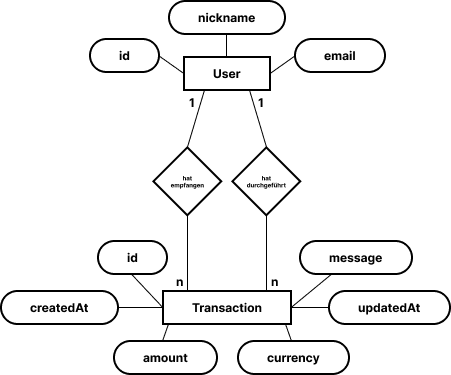
\includegraphics[width=.5\textwidth]{er-diagramm.png}
  \caption{Darstellung des Entity-Relationship-Diagramms für die Datenbank}
  \label{fig:er_diagramm}
\end{figure}

Als kleine Abweichung von diesem ER-Diagramm wird das eigentliche Schema so umgesetzt, dass nur die Relation Absender-Transaction abgebildet wird.
Der Empfänger einer Transaktion wird als freies String-Feld umgesetzt, da dieser so frei definiert werden kann.
Solange die Transaktionen im Rahmen des Projekts einen fixen Empfänger erreichen, ist man so flexibler in der Handhabung und kann einen Dummy-Empfänger wie z.B. die E-Mail-Adresse des Braintree-Accounts angeben.
\\
Das Backend wird einem Docker-Container gehostet, welcher mithilfe von Docker-Compose deployed werden kann.
\\
In Abbildung \ref{fig:apidesign} wird dargestellt, welche API-Endpunkte umgesetzt werden sollten:

\begin{figure}[H]
  \centering
  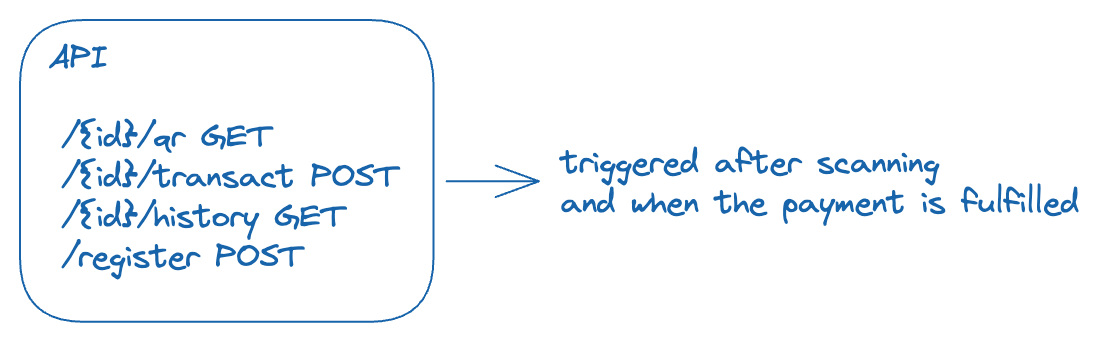
\includegraphics[width=.8\textwidth]{api-design.png}
  \caption{Darstellung der API-Endpunkte für das Backend}
  \label{fig:apidesign}
\end{figure}

Zunächst ist ein Endpunkt zur Registrierung vorgesehen, welcher dazu dient den Benutzer mithilfe eines Nicknames und einer E-Mail-Adresse zu registrieren.
Sofern ein Benutzer bereits existiert wird ein weiterer in der Datenbank angelegt, da hier keine Überprüfung stattfindet.
Dieser bekommt eine individuelle UUID zugeteilt und wird anschließend in der Datenbank gesichert.\\
\\
Es wurde an dieser Stelle bewusst auf eine reale Authentifizierung mittels bspw. Passwort und Session-ID oder JWT verzichtet, da so im Rahmen des Projekts auch auf das clientseitige Session-Handling verzichtet werden konnte.
So konnte an anderen Bestandteilen der App gearbeitet werden.\\
\\
Die UUID wird in den SharedPreferences der App gesichert und dient der Abfrage der weiteren Endpunkte.
Über den Endpunkt /{uuid}/history kann die Transaktionshistorie abgefragt werden.
Diese enthält alle Informationen über vergangene Transaktionen wie bspw. Betrag, Währung, Zeitpunkt und Empfänger.
Eine Transaktion wird clientseitig durch das Aufrufen des POST-Endpunkts /{uuid}/transact gesichert, sofern eine Zahlung komplett abgeschlossen wurde.
An diesen Endpunkt werden die o.g. Daten übergeben und diese so in der Datenbank gesichert.\\
\\
Der weitere Endpunkt /{uuid}/qr dient der Generierung eines individuellen QR-Codes, welcher jeweils für einen Benutzer generiert wird. Der QR-Code enthält einen vordefinierten Betrag, mithilfe dessen die Transaktionen gestartet werden können.
Als Weiterentwicklung der Applikation könnte so später eine echte Peer-To-Peer-Überweisung ermöglicht werden, sodass die scannende Person an denjenigen überweist, der den QR-Code mit seiner kodierten ID präsentiert.\\
\\
Der QR-Code kodiert folgende Informationen in Form eines JSON-Objekts:
\begin{lstlisting}[caption={Vom Backend generierte Notation für den QR-Code}]
  { namespace: "payero", id:{UUID}, amount: "2.0" }
\end{lstlisting}
Mithilfe des Namespace-Attributes kann geprüft werden, ob der QR-Code für Payero vorgesehen ist.
Ebenfalls enthält der QR-Code die Benutzer-UUID und den Betrag als Gleitkommazahl.

\subsection{Sicherheit}

Für eine produktive Nutzung der App sollte eine echte Authentifzierung über das Backend implementiert werden. Ebenso sollte sichergestellt werden, dass die QR-Codes nach der Erstellung nicht manipuliert werden können. Dies könnte etwa durch ein Public-Key-Verschlüsselungsverfahren sichergestellt werden. Als Implementierung könnten etwa JSON-Web-Tokens genutzt werden, die auf diesem Verfahren basieren. Ein weiterer Vorteil würde darin liegen, dass der QR-Code nicht beim Scannen mithilfe einer anderen App auslesbar wäre.
